\documentclass{ximera}
\graphicspath{  %% When looking for images,
{./}            %% look here first,
{./pictures/}   %% then look for a pictures folder,
{../pictures/}  %% which may be a directory up.
{../../pictures/}  %% which may be a directory up.
{../../../pictures/}  %% which may be a directory up.
{../../../../pictures/}  %% which may be a directory up.
}

\usepackage{listings}
%\usepackage{circuitikz}
\usepackage{xcolor}
\usepackage{amsmath,amsthm}
\usepackage{subcaption}
\usepackage{graphicx}
\usepackage{tikz}
%\usepackage{tikz-3dplot}
\usepackage{amsfonts}
%\usepackage{mdframed} % For framing content
%\usepackage{tikz-cd}

  \renewcommand{\vector}[1]{\left\langle #1\right\rangle}
  \newcommand{\arrowvec}[1]{{\overset{\rightharpoonup}{#1}}}
  \newcommand{\ro}{\texttt{R}}%% row operation
  \newcommand{\dotp}{\bullet}%% dot product
  \renewcommand{\l}{\ell}
  \let\defaultAnswerFormat\answerFormatBoxed
  \usetikzlibrary{calc,bending}
  \tikzset{>=stealth}
  




%make a maroon color
\definecolor{maroon}{RGB}{128,0,0}
%make a dark blue color
\definecolor{darkblue}{RGB}{0,0,139}
%define the color fourier0 to be the maroon color
\definecolor{fourier0}{RGB}{128,0,0}
%define the color fourier1 to be the dark blue color
\definecolor{fourier1}{RGB}{0,0,139}
%define the color fourier 1t to be the light blue color
\definecolor{fourier1t}{RGB}{173,216,230}
%define the color fourier2 to be the dark green color
\definecolor{fourier2}{RGB}{0,100,0}
%define teh color fourier2t to be the light green color
\definecolor{fourier2t}{RGB}{144,238,144}
%define the color fourier3 to be the dark purple color
\definecolor{fourier3}{RGB}{128,0,128}
%define the color fourier3t to be the light purple color
\definecolor{fourier3t}{RGB}{221,160,221}
%define the color fourier0t to be the red color
\definecolor{fourier0t}{RGB}{255,0,0}
%define the color fourier4 to be the orange color
\definecolor{fourier4}{RGB}{255,165,0}
%define the color fourier4t to be the darker orange color
\definecolor{fourier4t}{RGB}{255,215,0}
%define the color fourier5 to be the yellow color
\definecolor{fourier5}{RGB}{255,255,0}
%define the color fourier5t to be the darker yellow color
\definecolor{fourier5t}{RGB}{255,255,100}
%define the color fourier6 to be the green color
\definecolor{fourier6}{RGB}{0,128,0}
%define the color fourier6t to be the darker green color
\definecolor{fourier6t}{RGB}{0,255,0}

%New commands for this doc for errors in copying
\newcommand{\eigenvar}{\lambda}
%\newcommand{\vect}[1]{\mathbf{#1}}
\renewcommand{\th}{^{\text{th}}}
\newcommand{\st}{^{\text{st}}}
\newcommand{\nd}{^{\text{nd}}}
\newcommand{\rd}{^{\text{rd}}}
\newcommand{\paren}[1]{\left(#1\right)}
\newcommand{\abs}[1]{\left|#1\right|}
\newcommand{\R}{\mathbb{R}}
\newcommand{\C}{\mathbb{C}}
\newcommand{\Hilb}{\mathbb{H}}
\newcommand{\qq}[1]{\text{#1}}
\newcommand{\Z}{\mathbb{Z}}
\newcommand{\N}{\mathbb{N}}
\newcommand{\q}[1]{\text{``#1''}}
%\newcommand{\mat}[1]{\begin{bmatrix}#1\end{bmatrix}}
\newcommand{\rref}{\text{reduced row echelon form}}
\newcommand{\ef}{\text{echelon form}}
\newcommand{\ohm}{\Omega}
\newcommand{\volt}{\text{V}}
\newcommand{\amp}{\text{A}}
\newcommand{\Seq}{\textbf{Seq}}
\newcommand{\Poly}{\textbf{P}}
\renewcommand{\quad}{\text{    }}
\newcommand{\roweq}{\simeq}
\newcommand{\rowop}{\simeq}
\newcommand{\rowswap}{\leftrightarrow}
\newcommand{\Mat}{\textbf{M}}
\newcommand{\Func}{\textbf{Func}}
\newcommand{\Hw}{\textbf{Hamming weight}}
\newcommand{\Hd}{\textbf{Hamming distance}}
\newcommand{\rank}{\text{rank}}
\newcommand{\longvect}[1]{\overrightarrow{#1}}
% Define the circled command
\newcommand{\circled}[1]{%
  \tikz[baseline=(char.base)]{
    \node[shape=circle,draw,inner sep=2pt,red,fill=red!20,text=black] (char) {#1};}%
}

% Define custom command \strikeh that just puts red text on the 2nd argument
\newcommand{\strikeh}[2]{\textcolor{red}{#2}}

% Define custom command \strikev that just puts red text on the 2nd argument
\newcommand{\strikev}[2]{\textcolor{red}{#2}}

%more new commands for this doc for errors in copying
\newcommand{\SI}{\text{SI}}
\newcommand{\kg}{\text{kg}}
\newcommand{\m}{\text{m}}
\newcommand{\s}{\text{s}}
\newcommand{\norm}[1]{\left\|#1\right\|}
\newcommand{\col}{\text{col}}
\newcommand{\sspan}{\text{span}}
\newcommand{\proj}{\text{proj}}
\newcommand{\set}[1]{\left\{#1\right\}}
\newcommand{\degC}{^\circ\text{C}}
\newcommand{\centroid}[1]{\overline{#1}}
\newcommand{\dotprod}{\boldsymbol{\cdot}}
%\newcommand{\coord}[1]{\begin{bmatrix}#1\end{bmatrix}}
\newcommand{\iprod}[1]{\langle #1 \rangle}
\newcommand{\adjoint}{^{*}}
\newcommand{\conjugate}[1]{\overline{#1}}
\newcommand{\eigenvarA}{\lambda}
\newcommand{\eigenvarB}{\mu}
\newcommand{\orth}{\perp}
\newcommand{\bigbracket}[1]{\left[#1\right]}
\newcommand{\textiff}{\text{ if and only if }}
\newcommand{\adj}{\text{adj}}
\newcommand{\ijth}{\emph{ij}^\text{th}}
\newcommand{\minor}[2]{M_{#2}}
\newcommand{\cofactor}{\text{C}}
\newcommand{\shift}{\textbf{shift}}
\newcommand{\startmat}[1]{
  \left[\begin{array}{#1}
}
\newcommand{\stopmat}{\end{array}\right]}
%a command to give a name to explorations and hints and theorems
\newcommand{\name}[1]{\begin{centering}\textbf{#1}\end{centering}}
\newcommand{\vect}[1]{\vec{#1}}
\newcommand{\dfn}[1]{\textbf{#1}}
\newcommand{\transpose}{\mathsf{T}}
\newcommand{\mtlb}[2][black]{\texttt{\textcolor{#1}{#2}}}
\newcommand{\RR}{\mathbb{R}} % Real numbers
\newcommand{\id}{\text{id}}
\newcommand{\coord}[1]{\langle#1\rangle}
\newcommand{\RREF}{\text{RREF}}
\newcommand{\Null}{\text{Null}}
\newcommand{\Nullity}{\text{Nullity}}
\newcommand{\Rank}{\text{Rank}}
\newcommand{\Col}{\text{Col}}
\newcommand{\Ef}{\text{EF}}
\newcommand{\boxprod}[3]{\abs{(#1\times#2)\cdot#3}}

\author{Zack Reed}
%borrowed from ximera interactive la
\title{Determinants and Geometry}
\begin{document}
\begin{abstract}

\end{abstract}
\maketitle


\section*{Determinants, Areas, and Volumes}

So far, we've focused much of this chapter on determining properties of matrices and specifically whether or not they are invertible. 

We now introduce a very related topic that also has farther reaching implications for matrices as well, beyond invertibility, and is an important measure for Chapters 7, 8, and 9.

An intuition we've been discussing for whether matrices are invertibile is that when linear transformations ``squish'' space down to a smaller dimension, they are not invertible. One way to determine whether this ``squishing'' occurs is to measure by how much units of volume are stretched or compressed through the transformation. 

Consider, for instance, the matrix $\begin{bmatrix}
  3&0&0\\0&2&0\\0&0&1
\end{bmatrix}$. This stretches the $x$-axis by a factor of $3$ and the $y$-axis by a factor of $2$, as you can see in the following GeoGebra applet. Check the ``Adjust Matrix'' box and enter the columns of the matrix accordingly (note that the column vectors are listed as rows when being entered, so really you're entering the transpose of the matrix).

Then, select "Track Vector Transformation" to view the resulting transformation effect on singular vectors as well as the transformation of the unit cube. (RIGHT CLICK and drag to adjust the 3D view)

\begin{center}
  \geogebra{mdes5d4h}{858}{509}
\end{center}

As you can see, $A$ stretches out vectors in both the $x$ and $y$ directions while preserving the height. More importantly, the original $1\times1\times1$ cube becomes a stretched out rectangle, and the ``Transformed Volume'' measure reads as $6$. This means that the transformation stretches out space by a factor of $6$. 

If instead you enter the mug-squishing matrix $A=\begin{bmatrix}
  1&0&1\\0&2&2\\1&2&3
\end{bmatrix}$, you see the original cube squished down into a plane. 

The transformed volume of the unit cube is thus $\answer{0}$.

This gives us a clear way to determine whether linear transformations are invertible! Measuring this transformed volume is called finding \emph{the determinant}. The determinant arises from systematically extending the notions of areas and volumes to give clear ways of measuring volume-stretching and volume-compressing for any matrix transformation.

We will start with a $2$-dimensional approach to finding the area shifted by a transformation, and then build up to a $3$-dimensional volume shift. Higher-dimensional hypervolume shifts are just generlizations of what is done in $2$ and $3$ dimensions, and beyond $2$-dimensions the computations become rather cumbersome, so we will largely use MATLAB to compute determinants in practice. 

  \subsection*{Summary Video}
  Some people like to view summative videos at the beginning of an idea, some people like to get a summary at the end, some like both! If you want, before really digging in to the idea of the determinant, check out this video by Grant Sanderson! It'll be posted at the end of the discussion on Determinants as well, if you want to check it out then instead (or again).

  \begin{center}
    \youtube{Ip3X9LOh2dk}
\end{center}

    \subsection*{$2\times 2$ Determinant and the Area of a Parallelogram}
     
    Consider the parallelogram determined by vectors $\vec{u}$ and $\vec{v}$.
     
    \begin{center}
    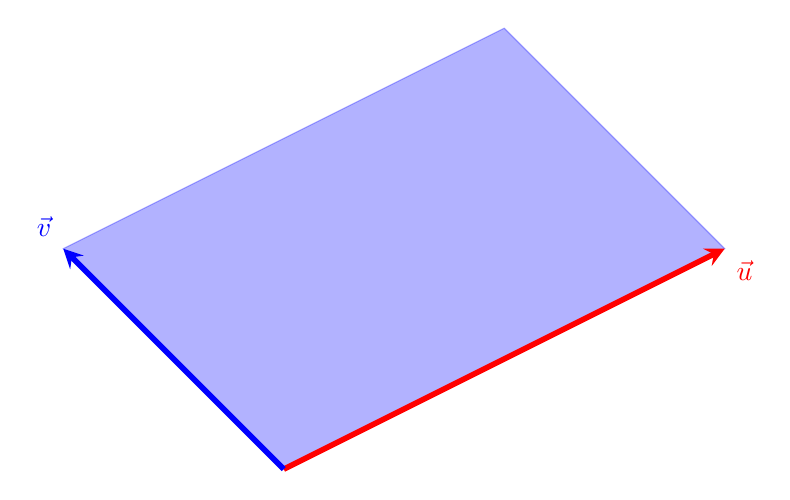
\begin{tikzpicture}[scale=1.4]
     
      \filldraw[blue, opacity=0.3](0,0)--(-2,2)--(2,4)--(4,2)--cycle;
     
    \draw[line width=2pt,red,-stealth](0,0)--(4,2) node[below right]{$\vec{u}$};
      
      \draw[line width=2pt,blue, -stealth](0,0)--(-2,2) node[above left]{$\vec{v}$};
    \end{tikzpicture}
    \end{center}

    $\vec{u}$ and $\vec{v}$ do not form a simple rectangle, and their orientation makes it initially cumbersome to get a parallelogram height and width for an area determination. 

    We can, however, cleverly set up a rectangular area from which we can use the coordinates of the vectors to determine the parallelogram area. This at first will be a bit laborious, but this process will work for any vector-spanning parallelogram and will also give us a means of defining the determinant!

    \begin{example}\label{ex:areaofparallelogram}
      First, let's draw the parallelogram within a grid.

      \begin{center}
      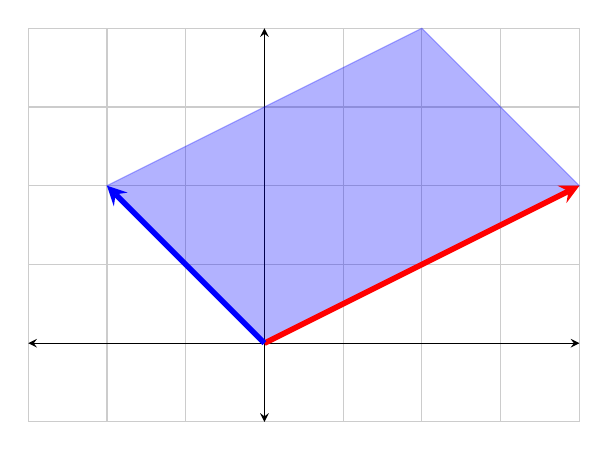
\begin{tikzpicture}[scale=1]
      \draw[thin,gray!40] (-3,-1) grid (4,4);
        \draw[<->] (-3,0)--(4,0);
        \draw[<->] (0,-1)--(0,4);
          
        \filldraw[blue, opacity=0.3](0,0)--(-2,2)--(2,4)--(4,2)--cycle;
        
      \draw[line width=2pt,red,-stealth](0,0)--(4,2);
        
        
       \draw[line width=2pt,blue,-stealth](0,0)--(-2,2);
         
      \end{tikzpicture}
      \end{center}

      \begin{explanation}

      The vectors that determine the parallelogram are
      $$\begin{bmatrix}4\\2\end{bmatrix}\quad\text{and}\quad\begin{bmatrix}-2\\2\end{bmatrix}$$

      The goal is to figure out the area of the parallelogram using just information from the two vectors. 

      As said earlier, we're going to put the parallelogram within a larger rectangle (using the vector coordinates), which will conveniently give us other geometric quantities from which we extract the paralellogram area!

      Let's create a rectangle that fully encompasses the parallelogram. The base of the rectangle will be the sum of the $x$-coordiantes, and the height will be the sum of the $y$-coordinates. This is true for any pair of vectors, and the key is that the vector $\vec{u}+\vec{v}$ determines the coordinates of the far tip. 

      Because this will generalize to any pair of vectors, let's use $\vec{u}=\begin{bmatrix}
        a\\c
      \end{bmatrix}$ and $\vec{v}=\begin{bmatrix}
        b\\d
      \end{bmatrix}$ as general stand-ins, and then at the end fill in our specific numbers.

      \begin{center}
        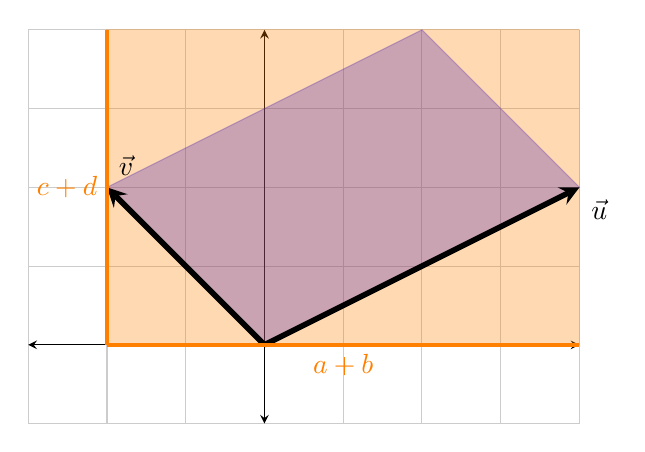
\begin{tikzpicture}[scale=1]
        \draw[thin,gray!40] (-3,-1) grid (4,4);
          \draw[<->] (-3,0)--(4,0);
          \draw[<->] (0,-1)--(0,4);
            
          \filldraw[blue, opacity=0.3](0,0)--(-2,2)--(2,4)--(4,2)--cycle;

              % Add the orange rectangle inscribing the parallelogram
          \filldraw[orange, opacity=.3] (-2,0) rectangle (4,4);

          \draw[line width=2pt,black,-stealth](0,0)--(4,2)node[below right]{$\vec{u}$};
            
           \draw[line width=2pt,black,-stealth](0,0)--(-2,2)node[above right]{$\vec{v}$};

             % Add thick orange lines for base and height
        \draw[orange, ultra thick] (-2,0) -- (4,0); % Base of the rectangle
        \draw[orange, ultra thick] (-2,0) -- (-2,4); % Height of the rectangle


        % Add labels
        \node[anchor=north, orange] at (1,0) {\(a+b\)}; % Label for the x-axis
        \node[anchor=east, orange] at (-2,2) {\(c+d\)}; % Label for the y-axis
           
        \end{tikzpicture}
        \end{center}

        Now, surrounding our parallelogram are four triangles, which actually break down quite nicely in terms of $a, b, c$, and $d$.

        The top left and bottom right triangles move along the vector $\vec{u}$, and so their dimensions come from the base $a$ and height $c$.

        \begin{center}
          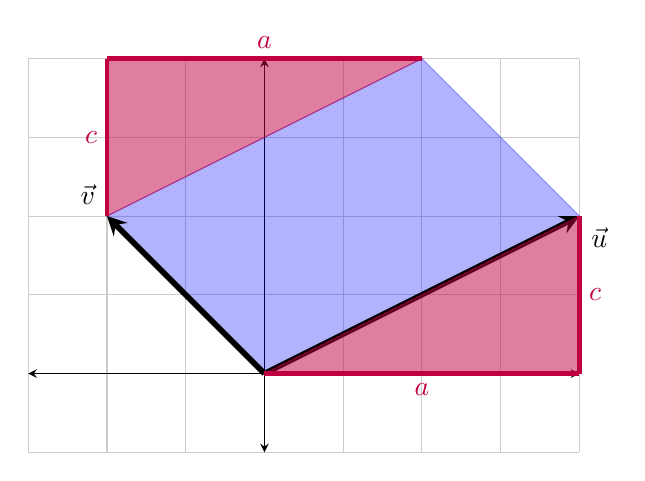
\begin{tikzpicture}[scale=1]
          \draw[thin,gray!40] (-3,-1) grid (4,4);
            \draw[<->] (-3,0)--(4,0);
            \draw[<->] (0,-1)--(0,4);
              
            \filldraw[blue, opacity=0.3](0,0)--(-2,2)--(2,4)--(4,2)--cycle;
  
                % Add the orange rectangle inscribing the parallelogram
            %\filldraw[orange, opacity=.3] (-2,0) rectangle (4,4);
            
          \draw[line width=2pt,black,-stealth](0,0)--(4,2)node[below right]{$\vec{u}$};
            
           \draw[line width=2pt,black,-stealth](0,0)--(-2,2)node[above left]{$\vec{v}$};
  
               % Add thick orange lines for base and height
          %\draw[orange, ultra thick] (-2,0) -- (4,0); % Base of the rectangle
          %\draw[orange, ultra thick] (-2,0) -- (-2,4); % Height of the rectangle

          % Add triangles to top-left and bottom-right corners
          \filldraw[purple, opacity=0.5] 
              (-2,4) -- (-2,2) -- (2,4) -- cycle; % Top-left triangle
          \draw[purple, ultra thick] (-2,4) -- (-2,2); % Thick edge for rectangle intersection
          \draw[purple, ultra thick] (-2,4) -- (2,4); % Thick edge for rectangle intersection

          \filldraw[purple, opacity=0.5] 
              (4,0) -- (4,2) -- (0,0) -- cycle; % Bottom-right triangle
          \draw[purple, ultra thick] (4,0) -- (4,2); % Thick edge for rectangle intersection
          \draw[purple, ultra thick] (4,0) -- (0,0); % Thick edge for rectangle intersection
  
  
          % Add labels
          \node[anchor=south, purple] at (0,4) {\(a\)}; % Label for the x-axis
          \node[anchor=north, purple] at (2,0) {\(a\)}; % Label for the x-axis
          \node[anchor=west, purple] at (4,1) {\(c\)}; % Label for the y-axis
          \node[anchor=east, purple] at (-2,3) {\(c\)}; % Label for the y-axis
             
          \end{tikzpicture}
          \end{center}

      Together, these triangles make a single rectangle of area $a\cdot c$. 

      Similarly, the top right and bottom left triangles of the orange rectangle make a rectangle of lencth $b\cdot d$, following the coordinates of $\vec{v}$. 

        \begin{center}
          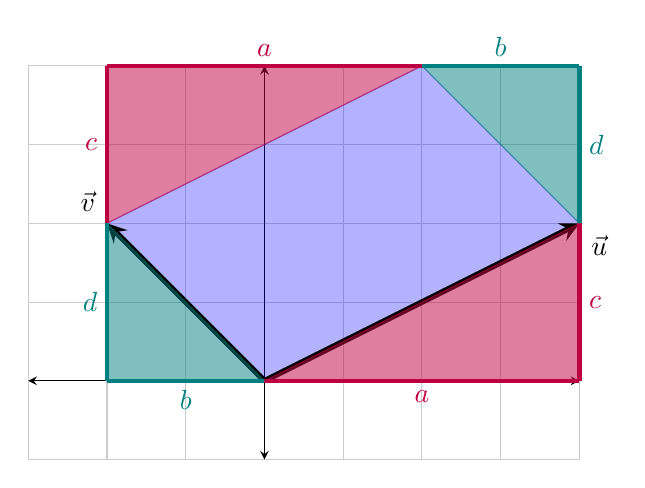
\begin{tikzpicture}[scale=1]
            % Draw grid and axes
            \draw[thin,gray!40] (-3,-1) grid (4,4);
            \draw[<->] (-3,0)--(4,0);
            \draw[<->] (0,-1)--(0,4);
            
            % Draw the parallelogram
            \filldraw[blue, opacity=0.3](0,0) -- (-2,2) -- (2,4) -- (4,2) -- cycle;
        
            % Draw vectors
            \draw[line width=2pt,black,-stealth](0,0) -- (4,2) node[below right] {\(\vec{u}\)};
            \draw[line width=2pt,black,-stealth](0,0) -- (-2,2) node[above left] {\(\vec{v}\)};
        
            % Add triangles to top-left and bottom-right corners
            \filldraw[purple, opacity=0.5] 
                (-2,4) -- (-2,2) -- (2,4) -- cycle; % Top-left triangle
            \draw[purple, ultra thick] (-2,4) -- (-2,2); % Thick edge for rectangle intersection
            \draw[purple, ultra thick] (-2,4) -- (2,4); % Thick edge for rectangle intersection
        
            \filldraw[purple, opacity=0.5] 
                (4,0) -- (4,2) -- (0,0) -- cycle; % Bottom-right triangle
            \draw[purple, ultra thick] (4,0) -- (4,2); % Thick edge for rectangle intersection
            \draw[purple, ultra thick] (4,0) -- (0,0); % Thick edge for rectangle intersection
        
            % Add triangles to top-right and bottom-left corners
            \filldraw[teal, opacity=0.5] 
                (4,4) -- (4,2) -- (2,4) -- cycle; % Top-right triangle
            \draw[teal, ultra thick] (4,4) -- (4,2); % Thick edge for rectangle intersection
            \draw[teal, ultra thick] (4,4) -- (2,4); % Thick edge for rectangle intersection
        
            \filldraw[teal, opacity=0.5] 
                (-2,0) -- (0,0) -- (-2,2) -- cycle; % Bottom-left triangle
            \draw[teal, ultra thick] (-2,0) -- (0,0); % Thick edge for rectangle intersection
            \draw[teal, ultra thick] (-2,0) -- (-2,2); % Thick edge for rectangle intersection
        
            % Add labels for purple triangles
            \node[anchor=south, purple] at (0,4) {\(a\)}; % Label for the top edge of the rectangle
            \node[anchor=north, purple] at (2,0) {\(a\)}; % Label for the bottom edge of the rectangle
            \node[anchor=west, purple] at (4,1) {\(c\)}; % Label for the right edge of the rectangle
            \node[anchor=east, purple] at (-2,3) {\(c\)}; % Label for the left edge of the rectangle
        
            % Add labels for teal triangles
            \node[anchor=west, teal] at (4,3) {\(d\)}; % Label for the top-right triangle edge
            \node[anchor=east, teal] at (-2,1) {\(d\)}; % Label for the bottom-left triangle edge
            \node[anchor=north, teal] at (-1,0) {\(b\)}; % Label for the bottom-left triangle edge
            \node[anchor=south, teal] at (3,4) {\(b\)}; % Label for the top-right triangle edge
          \end{tikzpicture}
        \end{center}

      Putting these areas together, we get the area of the parallelogram as the area of the large organge rectangle of base $b+a$ and height $c+d$, minus the two exterior rectangles (from the purple and teal triangles) of dimensions $a\times c$ and $b\times d$, respectively, to make:

      \begin{center}
        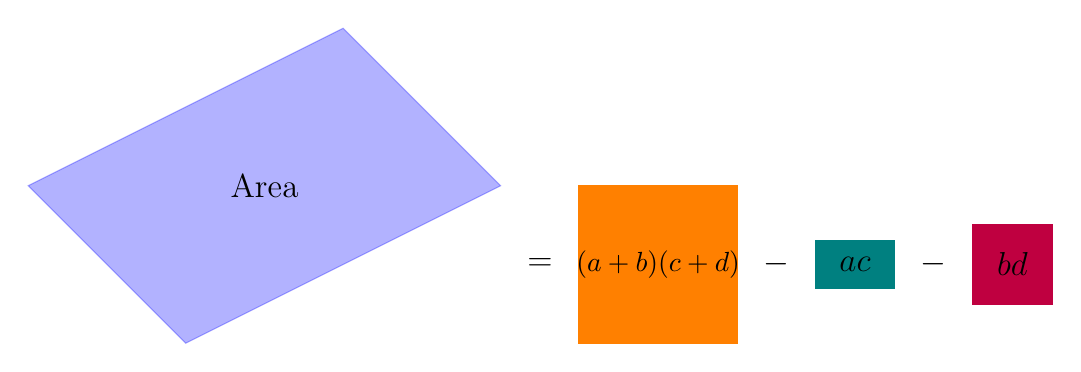
\begin{tikzpicture}[scale=1, every node/.style={font=\large}]
        
            % Draw the parallelogram
            \filldraw[blue, opacity=0.3](0,0) -- (-2,2) -- (2,4) -- (4,2) -- cycle;
            \node at (1,2) {\(\text{Area}\)};
            
            % Equal sign
            \node at (4.5,1) {\(=\)};
        
            % Yellow orange (a+b)(c+d)
            \filldraw[orange, thick] (5,0) rectangle (7,2);
            \node[font=\mdseries] at (6,1) {\((a+b)(c+d)\)};
            
            % Minus sign after yellow rectangle
            \node at (7.5,1) {\(-\)};
            
            % Green rectangle (ac)
            \filldraw[teal, thick] (8,0.7) rectangle (9,1.3);
            \node at (8.5,1) {\(ac\)};
            
            % Minus sign after green rectangle
            \node at (9.5,1) {\(-\)};
            
            % Blue rectangle (bd)
            \filldraw[purple, thick] (10,0.5) rectangle (11,1.5);
            \node at (10.5,1) {\(bd\)};
        
        \end{tikzpicture}
        \end{center}

      With one very important caveat, this means the area of the parallelogram is 

      $$\text{Area}=\abs{(a+b)(c+d)}-\abs{ac}-\abs{bd}=\abs{ad}+\abs{bc}$$

      As you can hopefully see, the caveat is that we need to put absolute value around each product to get the actual area. 

      If we look back at the particular diagram we're using, $b$ is a negative number, and lengths themselves cannot be negative. 

      If we were to write out the area accounting for the negative $b$ value, we would have

      $$\text{Area}=ad-bc.$$

      This is the determinant! Note that if both vectors are in the same quadrant, the geometric breakdown is a little more complicated but it works out to the same calculation.

  

      \end{explanation}
      \end{example}

        
      If we consider $\vec{u}$ and $\vec{v}$ as the columns of a matrix 

      $$A=\begin{bmatrix}
      a&c\\b&d
      \end{bmatrix},$$
      
      and want to ask ourselves the change in area under the transformation, we want the area of the resulting parallelogram from $\vec{u}$ and $\vec{v}$. 

      We use the notation $\mbox{det}(A)$ for ``the determinant of $A$'', as in the following definition:

      \begin{definition}
        The \emph{determinant} of a $2\times 2$ matrix $A=\begin{bmatrix}
          a&c\\b&d
        \end{bmatrix}$ is the computation 

        $$\mbox{det}(A)=ad-bc.$$

        This gives the \emph{signed} area of the paralellogram created by the columns of $A$. The \emph{unsigned} area of the paralellogram is $\abs{\mbox{det}(A)}$.
      \end{definition}

      \begin{remark}
        The reason that we clarify that $\mbox{det}(A)$ gives the signed area is the same as our need to clarify that we consider only lengths when dealing with areas. 

        The signs of the coordinates $a, b, c$, and $d$ are integral to the sign of the determinant $\mbox{det}(A)$, however the area measure itself remains the same.

        Getting a signed area is actually {\bf very} useful, however, as the sign of the determinant can tell us many things, much like how we also consider the sign of an integral to be an important bit of information beyond just giving us area.
      \end{remark}
        
        
      \begin{example}\label{exp:polyArea}
          Find the area of the polygon shown below. Do this by creating vectors to each of the polygon vertices, hence creating 5 triangles. Then use the determinant to find the areas of the resulting paralellograms (and then half that area for the triangles).
        \begin{center}
      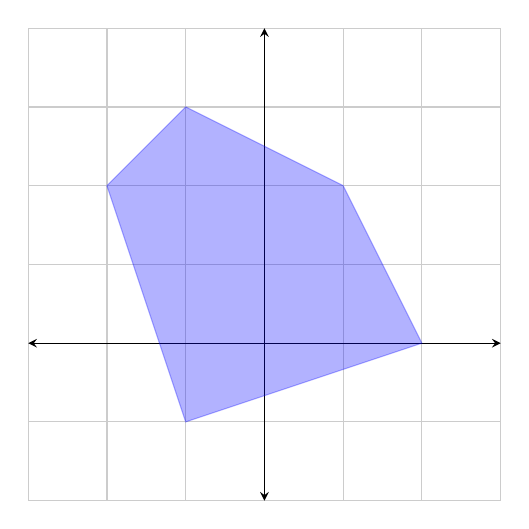
\begin{tikzpicture}[scale=1]
      \draw[thin,gray!40] (-3,-2) grid (3,4);
        \draw[<->] (-3,0)--(3,0);
        \draw[<->] (0,-2)--(0,4);
        \filldraw[blue, opacity=0.3](-1,-1)--(-2,2)--(-1,3)--(1,2)--(2,0)--cycle;
      %\draw[line width=2pt,red,-stealth](0,0)--(4,2);
      % \draw[line width=2pt,blue,-stealth](0,0)--(-2,2);
       \end{tikzpicture}
      \end{center}
      \begin{explanation}
          We will start by splitting this region into triangles.
          \begin{center}
      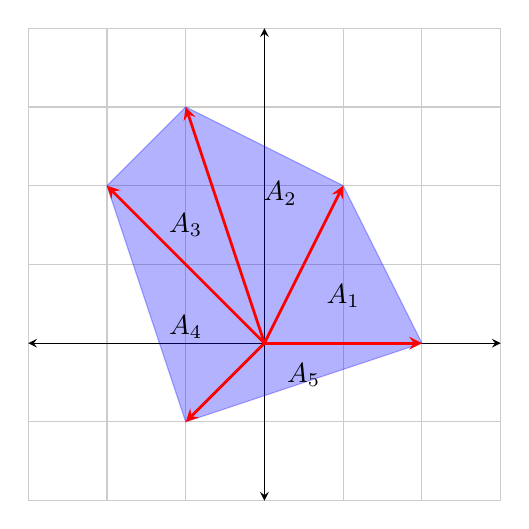
\begin{tikzpicture}[scale=1]
      \draw[thin,gray!40] (-3,-2) grid (3,4);
        \draw[<->] (-3,0)--(3,0);
        \draw[<->] (0,-2)--(0,4);
        \filldraw[blue, opacity=0.3](-1,-1)--(-2,2)--(-1,3)--(1,2)--(2,0)--cycle;
      \draw[line width=1pt,red,-stealth](0,0)--(-1,-1);
      \draw[line width=1pt,red,-stealth](0,0)--(-2,2);
      \draw[line width=1pt,red,-stealth](0,0)--(-1,3);
      \draw[line width=1pt,red,-stealth](0,0)--(1,2);
      \draw[line width=1pt,red,-stealth](0,0)--(2,0);
      \node[] at (1, 0.6)   (b) {$A_1$};
      \node[] at (0.2, 1.9)   (b) {$A_2$};
      \node[] at (-1, 1.5)   (b) {$A_3$};
      \node[] at (-1, 0.2)   (b) {$A_4$};
      \node[] at (0.5, -0.4)   (b) {$A_5$};
       \end{tikzpicture}
      \end{center}
          We can find the total area of the polygon by finding the area of each triangle.  The area of each triangle is half of the area of the corresponding parallelogram.  For instance, $A_1$ is half of the area of the parallelogram depicted below.
      \begin{center}
      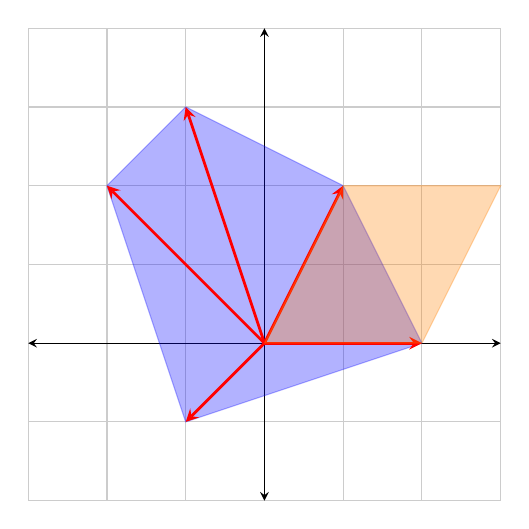
\begin{tikzpicture}[scale=1]
      \draw[thin,gray!40] (-3,-2) grid (3,4);
        \draw[<->] (-3,0)--(3,0);
        \draw[<->] (0,-2)--(0,4);
        \filldraw[blue, opacity=0.3](-1,-1)--(-2,2)--(-1,3)--(1,2)--(2,0)--cycle;
      \draw[line width=1pt,red,-stealth](0,0)--(-1,-1);
      \draw[line width=1pt,red,-stealth](0,0)--(-2,2);
      \draw[line width=1pt,red,-stealth](0,0)--(-1,3);
      \draw[line width=1pt,red,-stealth](0,0)--(1,2);
      \draw[line width=1pt,red,-stealth](0,0)--(2,0);
      \filldraw[orange, opacity=0.3](2,0)--(0,0)--(1,2)--(3,2)--cycle;
       \end{tikzpicture}
      \end{center}
      We compute
      $$A_1=\frac{1}{2}\left|\det\begin{bmatrix}2 & 1\\0 & 2\end{bmatrix}\right |=\answer{2}$$
      $$A_2=\frac{1}{2}\left|\det\begin{bmatrix}1 & -1\\2 & 3\end{bmatrix}\right |=\answer{2.5}$$
      $$A_3=\frac{1}{2}\left|\det\begin{bmatrix}-1 & -2\\3 & 2\end{bmatrix}\right |=\answer{2}$$
      $$A_4=\frac{1}{2}\left|\det\begin{bmatrix}-2 & -1\\2 & -1\end{bmatrix}\right |=\answer{2}$$
      $$A_5=\frac{1}{2}\left|\det\begin{bmatrix}-1 & 2\\-1 & 0\end{bmatrix}\right |=\answer{1}$$
      The total area of the polygon is $\answer{9.5}$.
      \end{explanation}
      \end{example}

  As a final exploration before generalizing into higher dimensions, let's explore two connections between inverses and the determinant. 

  First, we've discussed already that matrices which squish space down to a lower dimension are not invertible. In terms of the $2\times 2$ determinant, squishing down from area to lower dimensions means changing space into a line or just into a single dot at the origin. Either way, the resulting area is $0$ (a line or point has no area)! So, the determinant is $0$. Let's explore this.

  \begin{example}
    Find the determinant of the transformation represented by $A=\begin{bmatrix}
      1 &3\\2&6
    \end{bmatrix}$. 

    We can see that this squishes $\RR^2$ into the line with direction $\begin{bmatrix}
      1\\2
    \end{bmatrix}$, and is hence not invertible. 

    In terms of area, let's use the determinant to measure the area representing this transformation. 

    $$\mbox{det}(A)=\mbox{det}\left(\begin{bmatrix}
      1&3\\2&6
    \end{bmatrix}\right)=\answer{1}\cdot \answer{6}-\answer{3}\cdot \answer{2}=0.$$

    As we hoped, and as follows our geometric intuition, the determinant of $A$ is $0$, following the non-area of the resulting line.
  \end{example}

  This generally follows for any $n\times n$ matrix $A$, that a $0$ determinant is an indication of dimension-reduction in the transformation and hence $A$ is not invertible. Thus, even though we haven't defined the determinant for more than $2\times 2$ matrices yet, we will state the following theorem:

  \begin{theorem}
    An $n\times n$ matrix $A$ is invertible if and only if $\mbox{det}(A)\neq 0$. 
  \end{theorem}

  Finally, we also have an explicit way to calculate the inverse of a $2\times 2$ matrix using the determinant, though we will not go into its derivation.

  \begin{theorem}
    Let $A$ be a $2\times 2$ matrix $\begin{bmatrix}
    a&c\\b&d
    \end{bmatrix}$. If $\mbox{det}(A)\neq 0$, then $A^{-1}$ exists and is calculated as 

    $$A^{-1}=\frac{1}{\mbox{det}(A)}\begin{bmatrix}
      d &-b \\-c&a
    \end{bmatrix}.$$
  \end{theorem}

\end{document}